
\documentclass[letterpaper,hide notes,xcolor={table,svgnames},pdftex,10pt]{beamer}
\def\showexamples{t}


%\usepackage[svgnames]{xcolor}

%% Demo talk
%\documentclass[letterpaper,notes=show]{beamer}

\usecolortheme{crane}
\setbeamertemplate{navigation symbols}{}

\usetheme{MyPittsburgh}
%\usetheme{Frankfurt}

%\usepackage{tipa}

\usepackage{hyperref}
\usepackage{graphicx,xspace}
\usepackage[normalem]{ulem}
\usepackage{multicol}
\usepackage{amsmath,amssymb,amsthm,graphicx,xspace}
\newcommand\SF[1]{$\bigstar$\footnote{SF: #1}}

\usepackage[default]{sourcesanspro}
\usepackage[T1]{fontenc}
\usepackage[scaled]{beramono}
\usepackage{tikzpagenodes}

\newcounter{tmpnumSlide}
\newcounter{tmpnumNote}


% old question code
%\newcommand\question[1]{{$\bigstar$ \small \onlySlide{2}{#1}}}
% \newcommand\nquestion[1]{\ifdefined \presentationonly \textcircled{?} \fi \note{\par{\Large \textbf{?}} #1}}
% \newcommand\nanswer[1]{\note{\par{\Large \textbf{A}} #1}}


 \newcommand\mnote[1]{%
   \addtocounter{tmpnumSlide}{1}
   \ifdefined\showcues {~\tiny\fbox{\arabic{tmpnumSlide}}}\fi
   \note{\setlength{\parskip}{1ex}\addtocounter{tmpnumNote}{1}\textbf{\Large \arabic{tmpnumNote}:} {#1\par}}}

\newcommand\mmnote[1]{\note{\setlength{\parskip}{1ex}#1\par}}

%\newcommand\mnote[2][]{\ifdefined\handoutwithnotes {~\tiny\fbox{#1}}\fi
% \note{\setlength{\parskip}{1ex}\textbf{\Large #1:} #2\par}}

%\newcommand\mnote[2][]{{\tiny\fbox{#1}} \note{\setlength{\parskip}{1ex}\textbf{\Large #1:} #2\par}}

\newcommand\mquestion[2]{{~\color{red}\fbox{?}}\note{\setlength{\parskip}{1ex}\par{\Large \textbf{?}} #1} \note{\setlength{\parskip}{1ex}\par{\Large \textbf{A}} #2\par}\ifdefined \presentationonly \pause \fi}

\newcommand\blackboard[1]{%
\ifdefined   \showblackboard
  {#1}
  \else {\begin{center} \fbox{\colorbox{blue!30}{%
         \begin{minipage}{.95\linewidth}%
           \hspace{\stretch{1}} Some space intentionally left blank; done at the blackboard.%
         \end{minipage}}}\end{center}}%
         \fi%
}



%\newcommand\q{\tikz \node[thick,color=black,shape=circle]{?};}
%\newcommand\q{\ifdefined \presentationonly \textcircled{?} \fi}

\usepackage{listings}
\lstset{basicstyle=\footnotesize\ttfamily,
	breaklines=true,
	aboveskip=15pt,
  	belowskip=15pt,
	frame=lines,
	numbers=left, basicstyle=\scriptsize, numberstyle=\tiny, stepnumber=0, numbersep=2pt
}

\usepackage{siunitx}
\newcommand\sius[1]{\num[group-separator = {,}]{#1}\si{\micro\second}}
\newcommand\sims[1]{\num[group-separator = {,}]{#1}\si{\milli\second}}
\newcommand\sins[1]{\num[group-separator = {,}]{#1}\si{\nano\second}}
\sisetup{group-separator = {,}, group-digits = true}

%% -------------------- tikz --------------------
\usepackage{tikz}
\usetikzlibrary{positioning}
\usetikzlibrary{arrows,backgrounds,automata,decorations.shapes,decorations.pathmorphing,decorations.markings,decorations.text,decorations.pathreplacing}

\tikzstyle{place}=[circle,draw=blue!50,fill=blue!20,thick, inner sep=0pt,minimum size=6mm]
\tikzstyle{transition}=[rectangle,draw=black!50,fill=black!20,thick, inner sep=0pt,minimum size=4mm]

\tikzstyle{block}=[rectangle,draw=black, thick, inner sep=5pt]
\tikzstyle{bullet}=[circle,draw=black, fill=black, thin, inner sep=2pt]

\tikzstyle{pre}=[<-,shorten <=1pt,>=stealth',semithick]
\tikzstyle{post}=[->,shorten >=1pt,>=stealth',semithick]
\tikzstyle{bi}=[<->,shorten >=1pt,shorten <=1pt, >=stealth',semithick]

\tikzstyle{mut}=[-,>=stealth',semithick]

\tikzstyle{treereset}=[dashed,->, shorten >=1pt,>=stealth',thin]

\usepackage{ifmtarg}
\usepackage{xifthen}
\makeatletter
% new counter to now which frame it is within the sequence
\newcounter{multiframecounter}
% initialize buffer for previously used frame title
\gdef\lastframetitle{\textit{undefined}}
% new environment for a multi-frame
\newenvironment{multiframe}[1][]{%
\ifthenelse{\isempty{#1}}{%
% if no frame title was set via optional parameter,
% only increase sequence counter by 1
\addtocounter{multiframecounter}{1}%
}{%
% new frame title has been provided, thus
% reset sequence counter to 1 and buffer frame title for later use
\setcounter{multiframecounter}{1}%
\gdef\lastframetitle{#1}%
}%
% start conventional frame environment and
% automatically set frame title followed by sequence counter
\begin{frame}%
\frametitle{\lastframetitle~{\normalfont(\arabic{multiframecounter})}}%
}{%
\end{frame}%
}
\makeatother

\makeatletter
\newdimen\tu@tmpa%
\newdimen\ydiffl%
\newdimen\xdiffl%
\newcommand\ydiff[2]{%
    \coordinate (tmpnamea) at (#1);%
    \coordinate (tmpnameb) at (#2);%
    \pgfextracty{\tu@tmpa}{\pgfpointanchor{tmpnamea}{center}}%
    \pgfextracty{\ydiffl}{\pgfpointanchor{tmpnameb}{center}}%
    \advance\ydiffl by -\tu@tmpa%
}
\newcommand\xdiff[2]{%
    \coordinate (tmpnamea) at (#1);%
    \coordinate (tmpnameb) at (#2);%
    \pgfextractx{\tu@tmpa}{\pgfpointanchor{tmpnamea}{center}}%
    \pgfextractx{\xdiffl}{\pgfpointanchor{tmpnameb}{center}}%
    \advance\xdiffl by -\tu@tmpa%
}
\makeatother
\newcommand{\copyrightbox}[3][r]{%
\begin{tikzpicture}%
\node[inner sep=0pt,minimum size=2em](ciimage){#2};
\usefont{OT1}{phv}{n}{n}\fontsize{4}{4}\selectfont
\ydiff{ciimage.south}{ciimage.north}
\xdiff{ciimage.west}{ciimage.east}
\ifthenelse{\equal{#1}{r}}{%
\node[inner sep=0pt,right=1ex of ciimage.south east,anchor=north west,rotate=90]%
{\raggedleft\color{black!50}\parbox{\the\ydiffl}{\raggedright{}#3}};%
}{%
\ifthenelse{\equal{#1}{l}}{%
\node[inner sep=0pt,right=1ex of ciimage.south west,anchor=south west,rotate=90]%
{\raggedleft\color{black!50}\parbox{\the\ydiffl}{\raggedright{}#3}};%
}{%
\node[inner sep=0pt,below=1ex of ciimage.south west,anchor=north west]%
{\raggedleft\color{black!50}\parbox{\the\xdiffl}{\raggedright{}#3}};%
}
}
\end{tikzpicture}
}


%% --------------------

%\usepackage[excludeor]{everyhook}
%\PushPreHook{par}{\setbox0=\lastbox\llap{MUH}}\box0}

%\vspace*{\stretch{1}

%\setbox0=\lastbox \llap{\textbullet\enskip}\box0}

\setlength{\parskip}{\fill}

\newcommand\noskips{\setlength{\parskip}{1ex}}
\newcommand\doskips{\setlength{\parskip}{\fill}}

\newcommand\xx{\par\vspace*{\stretch{1}}\par}
\newcommand\xxs{\par\vspace*{2ex}\par}
\newcommand\tuple[1]{\langle #1 \rangle}
\newcommand\code[1]{{\sf \footnotesize #1}}
\newcommand\ex[1]{\uline{Example:} \ifdefined \presentationonly \pause \fi
  \ifdefined\showexamples#1\xspace\else{\uline{\hspace*{2cm}}}\fi}

\newcommand\ceil[1]{\lceil #1 \rceil}


\AtBeginSection[]
{
   \begin{frame}
       \frametitle{Outline}
       \tableofcontents[currentsection]
   \end{frame}
}



\pgfdeclarelayer{edgelayer}
\pgfdeclarelayer{nodelayer}
\pgfsetlayers{edgelayer,nodelayer,main}

\tikzstyle{none}=[inner sep=0pt]
\tikzstyle{rn}=[circle,fill=Red,draw=Black,line width=0.8 pt]
\tikzstyle{gn}=[circle,fill=Lime,draw=Black,line width=0.8 pt]
\tikzstyle{yn}=[circle,fill=Yellow,draw=Black,line width=0.8 pt]
\tikzstyle{empty}=[circle,fill=White,draw=Black]
\tikzstyle{bw} = [rectangle, draw, fill=blue!20, 
    text width=4em, text centered, rounded corners, minimum height=2em]
    
    \newcommand{\CcNote}[1]{% longname
	This work is licensed under the \textit{Creative Commons #1 3.0 License}.%
}
\newcommand{\CcImageBy}[1]{%
	\includegraphics[scale=#1]{creative_commons/cc_by_30.pdf}%
}
\newcommand{\CcImageSa}[1]{%
	\includegraphics[scale=#1]{creative_commons/cc_sa_30.pdf}%
}
\newcommand{\CcImageNc}[1]{%
	\includegraphics[scale=#1]{creative_commons/cc_nc_30.pdf}%
}
\newcommand{\CcGroupBySa}[2]{% zoom, gap
	\CcImageBy{#1}\hspace*{#2}\CcImageNc{#1}\hspace*{#2}\CcImageSa{#1}%
}
\newcommand{\CcLongnameByNcSa}{Attribution-NonCommercial-ShareAlike}

\newenvironment{changemargin}[1]{% 
  \begin{list}{}{% 
    \setlength{\topsep}{0pt}% 
    \setlength{\leftmargin}{#1}% 
    \setlength{\rightmargin}{1em}
    \setlength{\listparindent}{\parindent}% 
    \setlength{\itemindent}{\parindent}% 
    \setlength{\parsep}{\parskip}% 
  }% 
  \item[]}{\end{list}} 




% Custom packages
\usepackage{xcolor}
\definecolor{solarizedBase03}{HTML}{FFFFFF}
\definecolor{solarizedBase02}{HTML}{000000}
\definecolor{solarizedBase00}{HTML}{657B83}
\definecolor{solarizedBase0}{HTML}{000000}
\definecolor{solarizedBase1}{HTML}{93A1A1}
\definecolor{solarizedBase3}{HTML}{FDF6E3}


\usepackage[listings]{tcolorbox}
\newtcbinputlisting{\codelisting}[2][]{
    listing file={#2},
    colback=solarizedBase03,
    colframe=solarizedBase02,
    colupper=solarizedBase0,
    fonttitle=\bfseries\color{solarizedBase1},
    listing options={basicstyle=\ttfamily\footnotesize},
    listing only,
    #1
}
\newtheorem{defn}{Definition}

\title{Lecture 17 --- Early Termination, Reduced-Resource Computation }

\author{Patrick Lam \& Jeff Zarnett \\ \small \texttt{patrick.lam@uwaterloo.ca}, \texttt{jzarnett@uwaterloo.ca}}
\institute{Department of Electrical and Computer Engineering \\
  University of Waterloo}
\date{\today}


\begin{document}

\begin{frame}
  \titlepage

 \end{frame}


\begin{frame}
\frametitle{Quitting Time}

\begin{center}
	
\includegraphics[width=0.7\textwidth]{images/quitting-time.jpg}
\end{center}

Knowing when to quit is wise.

\end{frame}


\begin{frame}
\frametitle{Two Strategies}
There are two basic ideas. 

\begin{itemize}
\item Skip some parts of work
\item Intentionally reduce accuracy to speed things up. 
\end{itemize}

You may implement these strategies when you're writing an exam.

Your program might support only one.

\end{frame}



%%%%%%%%%%%%%%%%%%%%%%%%%%%%%%%%%%%%%%%%%%%%%%%%%%%%%%%%%%%%%%%%%%%%%%%%%%%%%%%%
\begin{frame}
  \frametitle{Early Phase Termination}



  We've seen barriers before.\\

  No thread may proceed past a barrier until all of the threads
reach the barrier.\\[1em]

  This may slow down the program: maybe one of the threads is horribly
  slow.\\[1em]

  Solution: kill the slowest thread.


\end{frame}
%%%%%%%%%%%%%%%%%%%%%%%%%%%%%%%%%%%%%%%%%%%%%%%%%%%%%%%%%%%%%%%%%%%%%%%%%%%%%%%%

%%%%%%%%%%%%%%%%%%%%%%%%%%%%%%%%%%%%%%%%%%%%%%%%%%%%%%%%%%%%%%%%%%%%%%%%%%%%%%%%
\begin{frame}
  \frametitle{Early Phase Termination: Objection}

\Huge
\begin{center}
``Oh no, that's going to change the meaning of the program!''
\end{center}
\end{frame}
%%%%%%%%%%%%%%%%%%%%%%%%%%%%%%%%%%%%%%%%%%%%%%%%%%%%%%%%%%%%%%%%%%%%%%%%%%%%%%%%

%%%%%%%%%%%%%%%%%%%%%%%%%%%%%%%%%%%%%%%%%%%%%%%%%%%%%%%%%%%%%%%%%%%%%%%%%%%%%%%%
\begin{frame}
  \frametitle{Early Phase Termination: When is it OK anyway?}


OK, so we don't want to be completely crazy.\\[1em]

Instead: 
\begin{itemize}
\item develop a statistical model of the program behaviour.
\item only kill tasks that don't introduce unacceptable distortions.
\end{itemize}

~\\[1em]

When we run the program: \\ \qquad get the output, plus a confidence interval.



\end{frame}
%%%%%%%%%%%%%%%%%%%%%%%%%%%%%%%%%%%%%%%%%%%%%%%%%%%%%%%%%%%%%%%%%%%%%%%%%%%%%%%%



\begin{frame}
\frametitle{Oh noooo!}

Example:
\begin{center}
	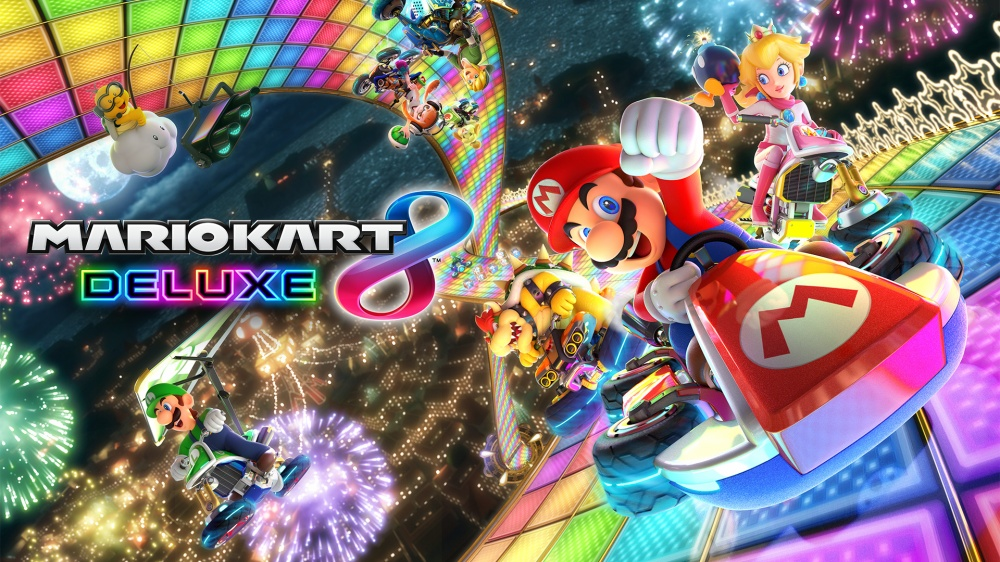
\includegraphics[width=0.8\textwidth]{images/mariokart.jpg}
\end{center}

\end{frame}



\begin{frame}
\frametitle{Remember, Remember...}

Many problems are mathematically hard in nature: to find the optimal solution you have to consider every possibility. 

Well, what this strategy presupposes is: don't.

\end{frame}


\begin{frame}
\frametitle{This Route Sucks}

Imagine the travelling salesperson problem, just for the sake of an example. 

There are $n$ points to visit and you want to minimize the amount of travel time. 

The only way to know if a solution is best is to consider every possible route.

One way we can know if we're wasting time is to remember previous outcomes.

\end{frame}


\begin{frame}
\frametitle{This Route Sucks}

The solution we're evaluating will have some travel cost in units (maybe kms). 

If the currently-accumulated cost in kms is larger than the total of the thus-far best solution, give up. 

Another idea?

\end{frame}

\begin{frame}
\frametitle{Close Enough is Good Enough}

Another approach is to stop as soon as you have a solution that's reasonable. 

If our target is to get total travel under 500 km then we can stop searching as soon as we find one that satisfies this constraint.

\end{frame}

\begin{frame}
\frametitle{You Have Ten Chances}

You can also choose to reduce the amount of effort by trying, say, five or ten different possibilities and seeing which of those is the best.

There's no guarantee you'll get an optimal solution.

Interesting to think about: what does Google Maps do?

\end{frame}

%%%%%%%%%%%%%%%%%%%%%%%%%%%%%%%%%%%%%%%%%%%%%%%%%%%%%%%%%%%%%%%%%%%%%%%%%%%%%%%%
\begin{frame}
  \frametitle{Trading Accuracy for Performance}


    Consider Monte Carlo integration.\\
    It illustrates a general tradeoff: accuracy vs performance.\\
  
    Martin Rinard generalized the accuracy vs performance tradeoff with:
      \begin{itemize}
        \item early phase termination [OOPSLA07]
        \item loop perforation [CSAIL TR 2009]
      \end{itemize}

\end{frame}
%%%%%%%%%%%%%%%%%%%%%%%%%%%%%%%%%%%%%%%%%%%%%%%%%%%%%%%%%%%%%%%%%%%%%%%%%%%%%%%%



%%%%%%%%%%%%%%%%%%%%%%%%%%%%%%%%%%%%%%%%%%%%%%%%%%%%%%%%%%%%%%%%%%%%%%%%%%%%%%%%
\begin{frame}
  \frametitle{Early Phase Termination: Two Examples}



Monte Carlo simulators: \\
Raytracers:
\begin{itemize}
\item already picking points randomly.
\end{itemize}

In both cases: spawn a lot of threads.\\[1em]
Could wait for all threads to complete;\\
or just compensate for missing data points,\\
assuming they look like points you did compute.


\end{frame}
%%%%%%%%%%%%%%%%%%%%%%%%%%%%%%%%%%%%%%%%%%%%%%%%%%%%%%%%%%%%%%%%%%%%%%%%%%%%%%%%



\begin{frame}
\frametitle{Calling the Election}

In other cases, some threads simply take too long, but we don't need all of them to produce a result. 

If we are evaluating some protocol where the majority wins, we can stop as soon as sufficient results have been returned.

\begin{center}
	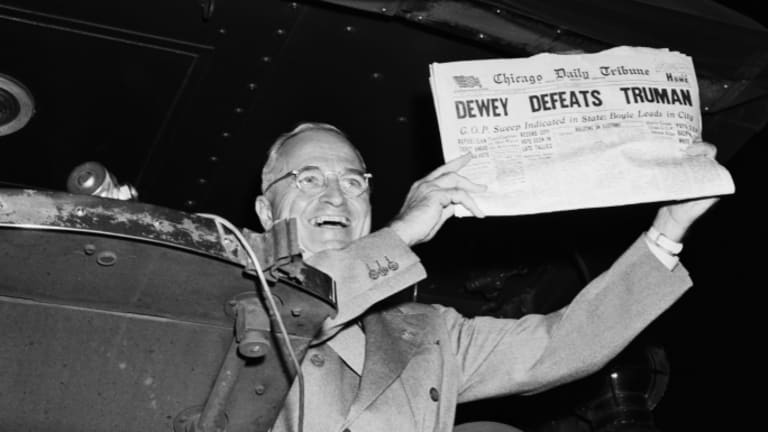
\includegraphics[width=0.5\textwidth]{images/dewey.jpg}
\end{center}


\end{frame}


\begin{frame}
\frametitle{A Solution Exists!}

For some categories of problem, we know not only that a solution will exist, but also how many steps it takes to solve (optimally). 

Consider the Rubik's Cube:

\begin{center}
	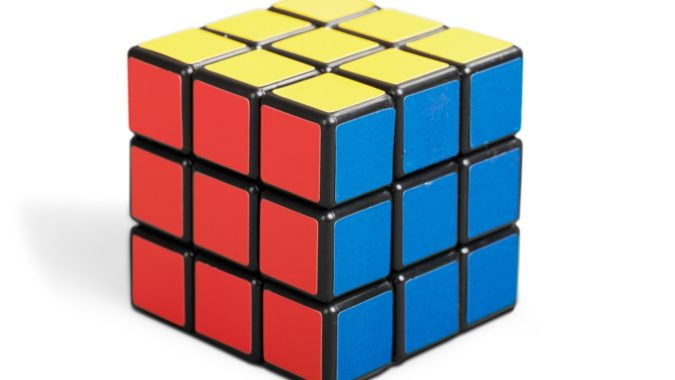
\includegraphics[width=0.4\textwidth]{images/rubikscube.jpg}
\end{center}

Brute force?

\end{frame}


\begin{frame}
\frametitle{Rubik's Cube}

Okay, that's fun to talk about, but it's always better if we see it in action? 

Let's play around with \url{https://rubiks-cube-solver.com/}

\end{frame}



\begin{frame}
\frametitle{Austerity Programs for Computer Programs}

We do more with less! 

Well, you can use \texttt{float} instead of \texttt{double}. 

But you can also work with integers to represent floating point numbers.

But when is it appropriate?


\end{frame}


\begin{frame}
\frametitle{Circuit Analysis}

You're entering points that were measured (with some error) and you're computing using machine numbers (also with some error).

The question is whether the simulation is good enough.

What resistors are going to be put in your circuit board?

is there any point in calculating it down to five decimal places when the resistors you buy have a tolerance of $\pm$5\%? 

\end{frame}


\begin{frame}
\frametitle{Circuit Analysis}


No, and if you took a circuits course with Prof. Barby he would be very disappointed if you said yes.

\begin{center}
	\includegraphics[width=0.5\textwidth]{images/barby.png}
\end{center}

\end{frame}


\begin{frame}
\frametitle{\texttt{iddqd}}

Quake III: ``fast inverse square root''. 

For graphics processing, sometimes you want to calculate $1/\sqrt{x}$.
.
Square root (or similar) is usually calculated by some interpolation or root-finding method

\end{frame}


\begin{frame}[fragile]
\frametitle{Fast Inverse Square Root}

\begin{lstlisting}[language=C]
float FastInvSqrt(float x) {
  float xhalf = 0.5f * x;
  int i = *(int*)&x;         // evil floating point bit level hacking
  i = 0x5f3759df - (i >> 1);  // what the fuck?
  x = *(float*)&i;
  x = x*(1.5f-(xhalf*x*x));
  return x;
}
\end{lstlisting}

 Now this probably seems like dark magic, and it is. 

\end{frame}


\begin{frame}
\frametitle{Float to Int?}

\begin{center}
	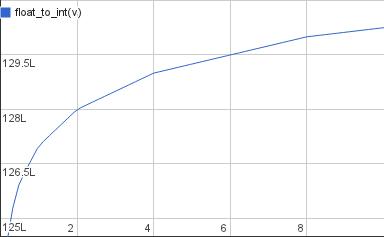
\includegraphics[width=0.4\textwidth]{images/float-to-int.png}
\end{center}



\end{frame}



\begin{frame}
\frametitle{Oh, never mind...}


The clever hack is somewhat obsoleted now by the fact that CPU instructions now exist to give you fast inverse square root. 

This was obviously not something you could rely on in 1999.

\end{frame}




\begin{frame}
\frametitle{The N-Body Simulation}

A common physics problem that programmers are asked to simulate is the N-Body problem.

\begin{center}
\includegraphics[width=0.8\textwidth]{images/Galaxy_Cluster_sim.png}
\end{center}
\hfill Image Credit: Michael L. Umbricht 


\end{frame}


\begin{frame}
\frametitle{Trade Accuracy for Performance}

You could look for optimizations that trade off accuracy for performance. 

As you might imagine, using \texttt{float} instead of \texttt{double}.


More? Then we need some domain knowledge. 

Hint: consider the formula: $F = \dfrac{Gm_{1}m_{2}}{r^{2}}$. 

\end{frame}



\begin{frame}
\frametitle{The N-Body Simulation}

Let's assume it's OpenCL converted and is optimized.

Can we use \texttt{float} instead of \texttt{double}?

What if we want more?

\end{frame}


\begin{frame}
\frametitle{Estimation is Okay}

Points that are far away contribute only very small forces. 

So you can estimate them (crudely). 

The idea is to divide the points into a number of ``bins'' which are cubes representing a locale of some sort. 

Then, compute the centre of mass for each bin. 

When calculating the forces: centre of mass for faraway bins; individual particles for nearby particles.


\end{frame}


\begin{frame}
\frametitle{This used to be an assignment... }

A more concrete explanation with an example: suppose the space  is divided into $[0, 1000]^3$, so we can take bins which are cubes of length 100. 

This gives 1000 bins. 

To increase the accuracy, what should we do?

To increase the speed, what should we do?

\end{frame}


\begin{frame}[fragile]
\frametitle{Compute Centre of Mass}

Compute all of the masses in parallel: create one thread per bin, and add a point's
position if it belongs to the bin:

\begin{lstlisting}
    int xbin, ybin, zbin; // initialize with bin coordinates
    int b;
    for (i = 0; i < POINTS; i++) {
        if (pts[i] in bin coordinates) {
            cm[b].x += pts[i].x; // y, z too
            cm[b].w += 1.0f;
        }
    }
    cm[b].x /= cm[b].w; // etc
\end{lstlisting}

Note that this parallelizes with the number of bins.


\end{frame}


\begin{frame}
\frametitle{Map Points}

For the next step, the program needs to keep track of the points in
each bin. 

 In a second phase,
iterate over all bins again, this time putting coordinates into the
proper element of {\tt binPts}, a two-dimensional array.

\end{frame}

\begin{frame}
\frametitle{Save Time}

The payoff from all these calculations is to save time while calculating forces. 

In this example, we'll compute exact forces for the points in the same bin and the directly-adjacent bins in each direction

That makes 27 bins in all, with 6 bins sharing a square, 12 bins sharing an edge, and 8 bins sharing a point with the centre bin). 

If there is no adjacent bin 
(i.e., this is an edge), just act as if there are no points 
in the place where the nonexistent bin would be. 

\end{frame}


\begin{frame}
\frametitle{More Overhead}

Necessarily, writing the program like this is going to mean more than one kernel.

This does mean there is overhead for each kernel, meaning the total amount of overhead goes up. 

Is it worth it? 

With 500*64 points:
\begin{itemize}
\item    OpenCL, no approximations (1 kernel): 0.182s
\item    OpenCL, with approximations (3 kernels): 0.168s
\end{itemize}

With 5000*64 points:
\begin{itemize}
\item    OpenCL, no approximations (1 kernel): 6.131s
\item    OpenCL, with approximations (3 kernels): 3.506s
\end{itemize}


\end{frame}




%%

%%%%%%%%%%%%%%%%%%%%%%%%%%%%%%%%%%%%%%%%%%%%%%%%%%%%%%%%%%%%%%%%%%%%%%%%%%%%%%%%
\begin{frame}[fragile]
  \frametitle{Loop Perforation}


  Like early-phase termination, but for sequential programs:\\
  \qquad throw away data that's not actually useful.

  \begin{lstlisting}
for (i = 0; i < n; ++i) sum += numbers[i];
  \end{lstlisting}

  \begin{center}
    $\Downarrow$
  \end{center}

  \begin{lstlisting}
for (i = 0; i < n; i += 2) sum += numbers[i];
sum *= 2;
  \end{lstlisting}

  This gives a speedup of $\sim$ 2 if {\tt numbers[]} is nice.\\[1em]

  Works for video encoding: can't observe difference.



\end{frame}
%%%%%%%%%%%%%%%%%%%%%%%%%%%%%%%%%%%%%%%%%%%%%%%%%%%%%%%%%%%%%%%%%%%%%%%%%%%%%%%%

%%%%%%%%%%%%%%%%%%%%%%%%%%%%%%%%%%%%%%%%%%%%%%%%%%%%%%%%%%%%%%%%%%%%%%%%%%%%%%%%
\begin{frame}
  \frametitle{Applications of Reduced Resource Computation}


  Loop perforation works for:
  \begin{itemize}
   \item evaluating forces on water molecules (summing numbers);
   \item Monte-Carlo simulation of swaption pricing;
   \item video encoding.
  \end{itemize}

  More on the video encoding example:\\
  Changing loop increments from 4 to 8 gives:
\begin{itemize}
 \item speedup of 1.67;
 \item signal-to-noise ratio decrease of 0.87\%;
 \item bitrate increase of 18.47\%;
 \item visually indistinguishable results.
\end{itemize}

\end{frame}

%%%%%%%%%%%%%%%%%%%%%%%%%%%%%%%%%%%%%%%%%%%%%%%%%%%%%%%%%%%%%%%%%%%%%%%%%%%%%%%%

%%%%%%%%%%%%%%%%%%%%%%%%%%%%%%%%%%%%%%%%%%%%%%%%%%%%%%%%%%%%%%%%%%%%%%%%%%%%%%%%
\begin{frame}[fragile]
  \frametitle{Video Encoding Skeleton Code}


\begin{lstlisting}
min = DBL_MAX;
index = 0;
for (i = 0; i < m; i++) {
  sum = 0;
  for (j = 0; j < n; j++) sum += numbers[i][j];
  if (min < sum) {
    min = sum;
    index = i;
  }
}
\end{lstlisting}
The optimization changes the loop increments and then compensates. 

\end{frame}

%%%%%%%%%%%%%%%%%%%%%%%%%%%%%%%%%%%%%%%%%%%%%%%%%%%%%%%%%%%%%%%%%%%%%%%%%%%%%%%%


\end{document}

